\chapter{MULTILAYER DRIPPING HANDRAIL}
\thispagestyle{empty}

Accretion disc model developed for the purpose of this study is constructed of $n$ times $m$ individual cells arranged in concentric circular grid, where $n$ is the number of concentric layers and $m$ number of cells in its layers. 

Each cell holds a set of parameters and its behavior is governed by set of oridinary differential equations derived from MSMM so fundamentally every cell is its own \emph{dripping faucet}. Layers move in the same direction\footnote{Direction is arbitrary and a matter of perspective (i.e. top vs. bottom view)} with keplerial orbital speeds relative to the outermost layer, which move by exacly one cell length in tangential direction in one simulation step. In every simulation step, there is a predefined constant mass influx into the outermost layer. This influx could come from specific azimuth or it could be distributed in some probabilistic manner from a wider range of angels.

As the simulation progresses the mass is distributed in tangential direction by the orbital movement of layers and in radial direction by overflow from individual cells. This radial mass transfer is unidirectional towards the grid center and is triggered by reaching a critical condition of MSMM in specific cells. 

Cell parameters and radial mass overflow are logged separately and later used to compute the radiative output, which is strongly dependent on radial mass transfer through changes in cell temperature and energy losses in gravitational potential of the imagined central body. 

Based on its characteristics this model is called a \emph{Multilayer Dripping Handrail} and hereinafter, it shall be referenced as MDH.

\section{MDH grid structure}

The cells are arranged in concentric circual grid of $n$ layers and $m$ cells in each layer. Layers are denoted by $i \in [0, n-1]$, with the outremost layer having the index $i = 0$. Individual cells in each layer are denoted by $j \in [0, m-1]$\footnote{Direction of $j$ index iteration is arbitrary and depends on inplementation}. Figure \ref{fig:initial_grid_state} shows simplified representation of this concentric simulation grid in its initial state. 

Whole simultaion grid acts like cellular automaton (CA). Cellular automata models usualy implement some kind of simple condition or set of conditions (e.g. Conway's game of life, see \cite{gardner1970}), to decide simulation development for the next step. In the case of model created by \cite{yonehara1997}, there is a simple mass limit condition triggering the radial mass trasfer. MDH takes this concept further and implements the condition as critical value of \emph{spring elongation} $z$ of MSMM, which is the solution of its ODE system solved repeatedly in every step. 

\begin{figure}
\centering
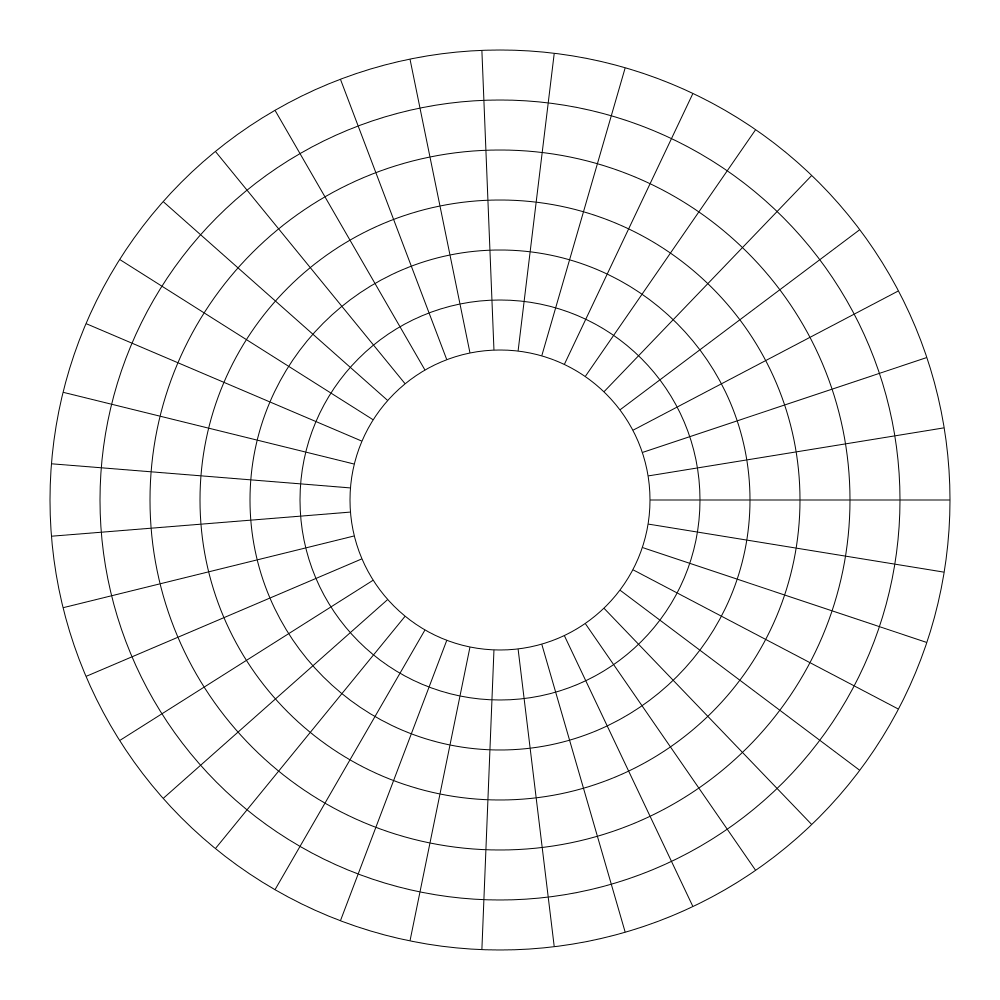
\includegraphics[width=0.9\columnwidth]{img/initial_grid_state.png}
\caption{Simplified representation of initial grid state}
\label{fig:initial_grid_state}
\end{figure}

\section{Cell definition}
Every cell holds following set of parameters:

\begin{center}
\begin{tabular}{r|l}
$i$			& Layer index \\
$j$			& Cell index \\
$r$			& Orbital radius \\
$\theta$	& Orbital azimuth \\ 
$z$			& Mass spring model \emph{spring elongation}  \\
$v$			& Mass-Spring model \emph{velocity} \\
$m$			& Mass contained by cell \\
$\Delta m$ 	& Mass change since previous step \\
$g$			& Gravitational acceleration relative to outermost layer \\
$\gamma$	& Constant Mass-Spring model dumpening parameter \\
$k$			& Mass-Spring model \emph{spring stiffness} \\
$T$			& Cell temperature \\ 
\end{tabular}
\end{center}

\begin{equation}
    \D{}{t} \left(m \D{z}{t}\right) = -kz - \gamma\D{z}{t} + mg,
\end{equation}

\begin{equation}
    \D{m}{t} = Q = const.,
\end{equation}



\subsection{Temperature}




\section{}
